\documentclass[border=3mm]{standalone}

\usepackage{tikz}


\begin{document}

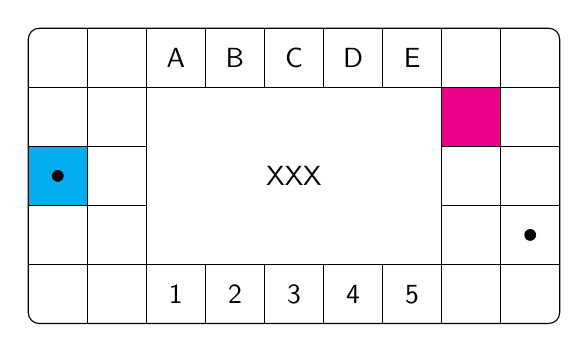
\begin{tikzpicture}[scale=.75,font=\sffamily]
    \begin{scope}[shift={(-.5,.5)}]
        \clip[draw,rounded corners] (-4,-3) rectangle (5,2);
        \fill[cyan] (-4,-1) rectangle +(1,1);
        \fill[magenta] (3,0) rectangle +(1,1);
        \draw (-4,-3) grid (5,2); 
        \draw[fill=white] (-2,-2) rectangle (3,1); 
    \end{scope}

    \fill (-4,0) circle(.1) (4,-1) circle(.1);

    \path node{XXX}
        (-2,2)   node{A} 
        ++(0:1)  node{B}
        ++(0:1)  node{C}
        ++(0:1)  node{D}
        ++(0:1)  node{E}
        
        (-2,-2)  node{1}          
        ++(0:1)  node{2}
        ++(0:1)  node{3}
        ++(0:1)  node{4}
        ++(0:1)  node{5};
\end{tikzpicture}

\end{document}